\documentclass{standalone}
\usepackage{pgfplots}
\pgfplotsset{compat=1.17}
\usetikzlibrary{arrows.meta}


\colorlet{green_set}{green!70!black}
\colorlet{purple_set}{blue!80!cyan!60!red!95!black!90}
\colorlet{red_set}{red!80!black}
\colorlet{orange_set}{orange!80!}

\begin{document}
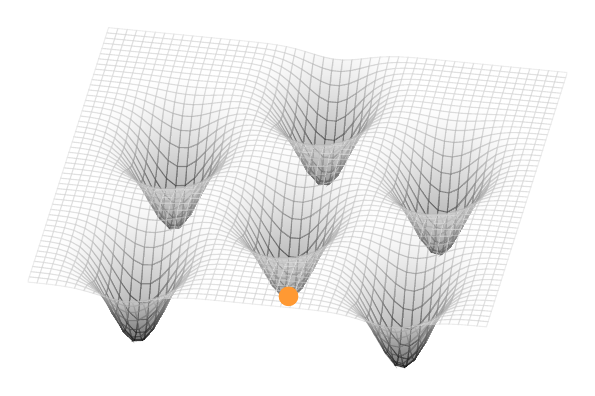
\begin{tikzpicture}
  \begin{axis}[
      view={10}{60},
      axis lines=none,
      domain=-3:3,
      set layers,
      y domain=-1.75:2.75,
      samples=50,
      zmax=1.5,
      z buffer=sort,
      colormap={greyscale}{gray(0cm)=(0); gray(1cm)=(1)},
    ]
    \addplot3 [surf, shader=faceted interp, opacity=0.35] 
    {   (1 - exp(-4*x^2 - 4*y^2)) *
        (1 - exp(-4*x^2 - 4*(y - 2)^2)) *
        (1 - exp(-4*(x + 2*sqrt(3)/2)^2 - 4*(y + 2/2)^2)) *
        (1 - exp(-4*(x + 2*sqrt(3)/2)^2 - 4*(y - 2/2)^2)) *
        (1 - exp(-4*(x - 2*sqrt(3)/2)^2 - 4*(y + 2/2)^2)) *
        (1 - exp(-4*(x - 2*sqrt(3)/2)^2 - 4*(y - 2/2)^2))
    };
    
    \coordinate (center) at (axis cs:0,0,0);
    \coordinate (green_top) at (axis cs:0,1,1);
    \coordinate (green_bottom) at (axis cs:0,2,0.05);
    \coordinate (purple_top) at (axis cs:{sqrt(3)/2},{-1/2},1);
    \coordinate (purple_bottom) at (axis cs:{2*sqrt(3)/2},-1,0.05);
    \coordinate (red_top) at (axis cs:{-sqrt(3)/2},{-1/2},1);
    \coordinate (red_bottom) at (axis cs:{-2*sqrt(3)/2},-1,0.05);

    \coordinate (up_right_bottom) at (axis cs:{2*sqrt(3)/2},1,0.05);
    \coordinate (up_right_top) at (axis cs:{2*sqrt(3)/2},0,1);
    \coordinate (up_left_bottom) at (axis cs:{-2*sqrt(3)/2},1,0.05);
    \coordinate (up_left_top) at (axis cs:{-2*sqrt(3)/2},0,1);

    \coordinate (red_top_opposite) at (axis cs:{-sqrt(3)/2},{3/2},1);
    \coordinate (purple_top_opposite) at (axis cs:{sqrt(3)/2},{1/2},1);

    \coordinate (coolio) at (axis cs:{sqrt(3)/2},{3/2},1);
    \coordinate (bobob) at (axis cs:{-sqrt(3)/2},{1/2},1);
  \end{axis}

\fill[orange_set] (center) circle (0.125);

\end{tikzpicture}
\end{document}
